\chapter{KAJIAN PUSTAKA}

\section*{ }
Demi mendukung penelitian ini, dibutuhkan beberapa teori penunjang sebagai bahan acuan dan referensi. 
Dengan demikian penelitian ini menjadi lebih terarah.
\vspace{1ex}

\section{Covid-19}

Covid-19 merupakan salah satu penyakit dengan daya penyebaran paling tinggi yang disebabkan oleh \textit{Severe
acute respiratory syndrome (SARS-CoV-2)}. Penyakit Covid-19 telah menyebabkan banyaknya korban jiwa serta kerugian
materi di berbagai aspek ekonomi. WHO menetapkan Covid-19 sebagai pandemi global pada tanggal 11 maret 2020. Pada
awalnya, dapat dikatakan bahwa pelayanan kesehatan tidak memiliki sistem yang baik dalam penanganan Covid-19.
Walaupun sistem pelayanan kesehatan terutama di rumah sakit dalam menangangi Covid-19 semakin lama semakin membaik
dan telah mengalami banyak kemajuan, beberapa mutasi yang mengubah karakteristik virus secara drastis dapat menimbulkan
semakin banyak korban jiwa maupun kerugian materi. Oleh karena itu pembatasan penyebaran virus dan variannya 
harus tetap dilakukan.

Hingga saat ini varian SARS-CoV-2 yang disebabkan oleh mutasi virus tetap terus diteliti, beberapa varian yang 
dianggap membahayakan karena meningkatnya daya penularan dan keagresifan virus diberi nama \textit{Variant 
of Concern (VOC)}.
Pada tanggal 11 Desember 2021, WHO menetapkan adanya lima \textit{variant of concern} yaitu :

\begin{enumerate}
    \item \textbf{Alpha (B.1.1.7)} 
    
    Varian Alpha merupakan \textit{variant of concern} pertama yang muncul di Inggris pada akhir Desember 2020 
    \cite{pmid33476315}. Varian ini memiliki 17 mutasi dan mempunyai peningkatan pada daya lekat ke sel 
    \textit{host} \cite{pmid33501442, pmid33658326}. Varian ini memiliki peningkatan transmisi 43\% Hingga
    82\% dibandingkan varian SARS-CoV-2 sebelumnya \cite{pmid33658326}. 

    \item \textbf{Beta (B.1.351)} 
    
    Varian Beta pertama kali dilaporkan di Afrika Selatan pada Desember 2020 dan menyebabkan adanya gelombang 
    kedua pandemi Covid-19 di Afrika Selatan \cite{pmid33690265}. Varian ini memiliki 9 mutasi \cite{pmid33630820}
    dimana varian ini memiliki kemampuan untuk menurunkan antibodi sehingga dapat menginfeksi orang yang telah
    divaksin atau menerima plasma konvalesen \cite{pmid33688656}.
    
    \item \textbf{Gamma(P.1)} 
    
    Varian Gamma pertama kali dilaporkan di Brazil pada awal Januari 2021 \cite{pmid33688664}. Varian Gamma
    memiliki 10 mutasi. Efek dari mutasi ini hampir mirip dengan varian Beta dimana varian ini memiliki kemampuan
    untuk menurun antibodi orang yang terinfeksi \cite{pmid33688656}.

    \item \textbf{Delta (B.1.617.2)}
    
    Varian Delta pertama kali dilaporkan di India pada Desember 2020. Varian ini merupakan salah satu yang paling
    berbahaya karena pasien yang terkena oleh varian delta mempunyai peluang kematian 133\% lebih tinggi dibandingkan
    varian awal dan 235\% lebih memungkinkan untuk masuk ke ruang ICU. Vaksin yang diberikan juga mengalami penurunan
    efektivitas melawan varian delta \cite{pmid34698149}.

    \item \textbf{Omicron (B.1.1.529)} 
    Varian Omicron pertama kali dilaporkan di Afrika Selatan pada November 2021 \cite{pmid34876769}. Varian 
    Omicron mempunyai 30 mutasi \cite{pmid34860154} dan 2,8 kali lebih menular dibandingkan varian delta. 

\end{enumerate}

\subsection{Cara Penularan}
Penyakit Covid-19 yang disebabkan oleh SARS-CoV-2 dapat menular melalui cara-cara berikut :

\begin{itemize}
    \item Transmisi SARS-CoV-2 yang paling umum ialah melalui paparan \textit{droplet} yang dikeluarkan oleh
    individu lain yang telah terinfeksi oleh virus tersebut.

    \item Melalui material seperti besi dan plastik yang terpapar oleh SARS-CoV-2, SARS-CoV-2 dapat bertahan 
    selama 72 jam pada material besi dan plastik, 24 jam pada material kardus, dan 4 jam pada material tembaga.
    Tingkat kontaminasi semakin meningkat jika barang tersebut digunakan oleh orang banyak contoh seperti tetikus
    komputer di rumah sakit \cite{pmid32275497}.

    \item Melalui transmisi vertikal dari ibu yang hamil kepada bayi yang akan dilahirkan, namun kasus ini jarang 
    terjadi, sebuah penelitian \cite{pmid32739398} mengungkapkan bahwa dari 936 bayi yang dilahirkan dari ibu yang positif Covid-19,
    hanya 27 bayi yang dinyatakan positif Covid-19.

\end{itemize}

\subsection{Epidemiologi}
Dari tulisan sebelumnya, sudah dapat diketahui bahwa Covid-19 dapat menimbulkan kematian, namun terdapat 
beberapa faktor yang mempengaruhi apakah pasien akan sembuh dari Covid-19 atau tidak. Beberapa faktor tersebut
adalah umur, gender, dan penyakit yang diderita oleh pasien. Pasien yang mempunyai umur di atas 65 tahun mempunyai
kemungkinan untuk meninggal lebih besar dibandingkan kelompok usia lain \cite{pmid33356661}. Penelitian lain
\cite{pmid32555134} mengakatakan bahwa pasien-pasien Covid-19 yang memiliki obesitas, penyakit jantung, penyakit
kronis ginjal, diabetes, penyakit kronis paru-paru, kanker, dan kebiasaan merokok lebih berpeluang untuk dirawat
di rumah sakit (45,4\%) dibandingkan yang tidak memiliki kondisi tersebut (7,6\%). Selain itu pasien-pasien
yang memiliki kondisi tersebut 12x lebih berpotensi untuk tidak sembuh dan meninggal (19,5\%) dibandingkan pasien
yang tidak memiliki kondisi kesehatan tersebut (1,6\%).

Kemudian jika dibedakan berdasarkan gender, berdasarkan data yang diperoleh, pasien pria lebih memiliki risiko
yang lebih tinggi untuk menjadi pasien Covid-19 dan meninggal akibat Covid-19 dibandingkan pasien perempuan 
\cite{pmid32450906}. Peneliti pun juga meniliti apakah ras dan etnik mempunyai hubungan dengan Covid-19. Hasil
dari meta-analisis peneliti Amerika dan Inggris mengatakan bahwa orang-orang dengan ras afrika, hispanik (keturunan eropa),
dan orang asia memiliki kecenderungan untuk mengalami Covid-19 \cite{pmid33200120}, dimana tingkat kematian 
tertinggi terjadi pada orang hispanik \cite{pmid33830988}.

\subsection{Dampak Covid-19}
Sangat banyak dampak negatif yang diberikan saat terjadinya pandemi Covid-19, jumlah korban jiwa karena kejadian
ini telah mencapai lebih dari 6 juta orang \cite{WHO}. Pandemi Covid-19 juga membawa dampak kemiskinan di berbagai
negara. Di awal pandemi Covid-19, masyarakat di beberapa negara melakukan \textit{panic buying} \cite{CHEN2022102970}.
Tindakan \textit{panic buying} ini terjadi karena ketakutan dari masyarakat untuk melakukan aktivitas di luar dan
kepanikan masyarakat dalam rangka bertahan hidup. Hal ini pun secara otomatis meningkatkan kelangkaan bahan makanan serta harga dari kebutuhan pokok sehari-hari.
Tingkat kemiskinan yang naik dan kelangkaan bahan makanan pun dapat dikatakan terjadi karena pandemi Covid-19 
\cite{HEADEY2022100626}. Tidak hanya kesehatan jasmani yang menjadi ancaman, beberapa penelitian juga membahas mengenai
dampak Covid-19 pada kesehatan mental masyarakat \cite{CAMPOARIAS2022114337}. Covid-19 memberikan dampak depresi
stress, dan trauma terutama pada masyarakat golongan bawah. Diskriminasi terhadpa pasien Covid-19 yang sembuh pun
turut mendukung kemungkinan terjadinya stress dan depresi pada orang yang sembuh dari penyakit Covid-19.

Dalam segi ekonomi, Covid-19 telah memberikan penurunan yang drastis pada pasar saham, performa industri, serta
menurunkan jumlah pembeli di pasar-pasar tradisional maupun modern. Pada pasar saham, penurunan indeks saham yang
terjadi pun berkolerasi erat dengan tingkat kasus Covid-19 yang terjadi \cite{UDEAJA2022e01076}. Penurunan nilai
saham ini pun dapat dikatakan terjadi berbagai belahan dunia. Performa yang menurun juga dialami oleh berbagai industri
mulai dari industri kreatif \cite{KHLYSTOVA20221192} hingga industri-industri besar \cite{XU202287}.

\subsection{Cara Penanggulangan}
Cara penanggulangan (termasuk cara pencegahan) Covid-19 dibedakan menjadi dua macam, yaitu dengan interfensi memprediksi
dan non-interfensi medis. Interfensi medis membahas mengenai penanganan Covid-19 yang meliputi penggunaan terapi medis,
obat-obatan, dan vaksinasi. Sedangkan non-interfensi medis membahasa mengenai regulasi maupun penyuluhan
bagi masyarakat.

\begin{itemize}
    \item \textbf{Penanganan Medis}
    
        Penanganan pandemi Covid-19 saat ini telah dilakukan dengan cara vaksinasi dan pemberian \textit{booster}
        pada masyarakat untuk meningkatkan daya tahan tubuh dan menurunkan efek negatif yang diberikan oleh virus
        SARS Cov-2 kepada tubuh penerima vaksin. Pemberian vaksin Covid-19 yang dilakukan secara umum telah memberikan efek melindungi 
        tubuh manusia serta memberikan kasiat klinis terhadap SARS-CoV 2 setidaknya 60\% bergantung pada jenis
        vaksin yang diberikan. Salah satu vaksin yang memberikan efek paling baik salah satunya adalah vaksin
        BNT162b2 yang lebih kita kenal sebagai vaksin pfizer mempunyai efektivitas 95\% terhadap penerima vaksin 
        kedua \cite{pmid33301246}.

        Penanganan Medis lainnya khususnya penanganan yang digunakan saat pasien terkena Covid-19 adalah terapi
        plasma konvalesen. Walaupun terapi ini diperbolehkan, terdapat beberapa penelitian yang memberikan data
        bahwa terapi plasma konvalesen tidak lebih baik dibandingkan dengan terapi pada umumnya \cite{pmid33232588,pmid32492084}.
        Pemberian antibodi juga dapat membantu pasien khususnya REGN-COV2 dan VIR-7831 sangat dianjurkan. antibodi
        REGN-COV2 menurunkan jumlah pasien yang meninggal hingga 70\% \cite{pmid33332778}, sedangkan antibodi 
        VIR-7831 menurunkan kemunungkinan pasien meninggal atau perlu dirawat di rumah sakit hingga 80\%. 

    \item \textbf{Penanganan Non Medis}
    
        Beberapa penanganan non medis pada pandemi Covid-19 juga telah dilaksanakan, beberapa hal penting yang dilakukan
        sebagai upaya penanganan non medis adalah penggunaan masker dan menjaga jarak satu sama lain. Penelitian \cite{HANTHANANARACHCHILAGE2021111458}
        mengatakan bahwa dengan menjaga jarak dan menggunakan masker, menurunkan persentasi prediksi terjadinya korban
        jiwa 25\% hingga 45\%. Penanganan ini merupakan hal yang termudah untuk dilakukan dalam menurunkan kasus
        Covid-19 yang terjadi. Penanganan non medis juga dapat dilakukan dengan cara menutup bandara, membatasi 
        kegiatan pariwisata, dan menutup beberapa tempat pusat kegiatan masyarakat \cite{GE2022102649}.

\end{itemize}

\section{Machine Learning}

\textit{Machine Learning} atau Pembelajaran Mesin adalah salah satu cabang dalam kecerdasan buatan dan ilmu 
komputer yang menggunakan data dan algoritma untuk meniru manusia dalam mempelajari sesuatu \cite{ibm_ml_expl}. 
Salah satu hal yang membuat pembelajaran mesin sangat diminati adalah kemampuannya untuk menyelesaikan suatu 
tugas dengan sedikit intervensi dari manusia.

Sekarang ini, pembelajaran mesin adalah salah satu fokus yang cukup diminati pada bidang \textit{data science}. 
Dimana dengan menggunakan pembelajaran mesin, diharapkan suatu kecerdasan buatan dapat menyelesaikan beberapa 
tugas yang bagi komputer cukup rumit seperti misalnya, memberikan prediksi yang akurat berdasarkan data, 
melakukan klasifikasi pada teks maupun pada gambar, melakukan pemrosesan citra guna mengenali objek di dalam 
citra tersebut, dan masih banyak lagi.

Untuk prosesnya sendiri, awalnya kita harus mengumpulkan data, data ini dapat kita ambil dari  berbagai sumber 
atau bisa juga menggunakan data yang berasal dari instansi atau pribadi (data yang kita buat sendiri). 
Selanjutnya adalah proses \textit{training} dimana data akan dimasukkan ke dalam model pembelajaran mesin 
yang sudah dipilih. Kita dapat merubah beberapa parameter dari model tersebut untuk meningkatkan akurasi dari 
suatu model pembelajaran mesin. Terakhir adalah melakukan proses \textit{testing}, dimana model akan melakukan 
prediksi pada set data yang berbeda dari yang digunakan pada saat proses \textit{training}. Apabila ternyata 
tingkat akurasi dirasa kurang memadai, dapat dilakukan proses \textit{re-training} sampai tingkat akurasi 
nya dirasa cukup. Hasil akhir dari proses ini adalah sebuah model pembelajaran mesin yang dapat digunakan 
walaupun menggunakan data yang berbeda \cite{mit_ml_expl}.

\subsection{\textit{Supervised Learning}}
Salah satu cabang dalam bidang pembelajaran mesin. Disini data yang dijadikan masukan ke model sudah diberikan 
label atau struktur tertentu \cite{ms_ml_expl}. Berdasarkan dari data berlabel tersebut, sebuah model akan 
merubah parameter internalnya agar mendekati atau sesuai dengan label yang diberikan \cite{ibm_ml_expl}. 
Salah satu contoh model pembelajaran mesin dengan metode pembelajaran seperti ini adalah \textit{Linear 
Regression, Random Forest}, dan sebagainya.

\subsection{\textit{Unsupervised Learning}}
Salah satu cabang dalam bidang pembelajaran mesin. Disini data yang dijadikan masukan ke model tidak diberikan 
label sama sekali. Nantinya model akan membuat pengelompokan (\textit{clusters}) dan hubungan berdasarkan dari 
data yang diberikan \cite{mit_ml_expl}. Contoh model yang menggunakan metode pembelajaran ini adalah 
\textit{K-NN clustering}.

\subsection{\textit{Reinforcement Learning}}
Salah satu cabang dalam bidang pembelajaran mesin. Disini model tidak diberikan data awal sama sekali, 
namun, model dibiarkan melakukan proses percobaan secara mandiri terus-menerus sampai tercapai hasil atau 
respon yang diinginkan. Apabila terdapat parameter yang menghasilkan respon positif, maka parameter tersebut 
disimpan dan digunakan sebagai masukan untuk iterasi \textit{training} berikutnya \cite{mit_ml_expl}.

\section{\textit{Deep Learning}}

Mirip seperti pembelajaran mesin, \textit{Deep Learning} juga merupakan salah satu bidang dalam bidang 
kecerdasan buatan. Yang membedakan antara pembelajaran mesin biasa dengan \textit{deep learning} adalah 
\textit{deep learning} mengacu pada penggunaan \textit{layer} dan \textit{artificial neural network} hingga
mempunyai \textit{multiple hidden layer}, sedangkan \textit{machine learning} lebih mengacu kepada seluruh 
algoritma yang dapat diterapkan untuk menemukan \textit{rules} dari serangkaian data. 
Keuntungan dari model jenis ini adalah model ini dapat memproses masukan yang paling 
abstrak sekalipun, sehingga menghilangkan proses ekstraksi fitur secara manual \cite{mathwork_deeplearning}. 
Namun, karena \textit{deep learning} memiliki \textit{layers} yang sangat banyak, maka diperlukan jumlah data 
yang jauh lebih banyak pula. Karena itu, sebuah model \textit{deep learning} memerlukan daya komputasi 
yang jauh lebih besar dibandingkan dengan model pembelajaran mesin biasa. Setiap \textit{layer} dapat 
memiliki fungsi dan tanggung jawabnya masing - masing \cite{mit_ml_expl}, seperti misal apabila kita 
menggunakan \textit{deep learning} untuk mendeteksi angka plat nomor di kendaraan bermotor, bisa saja beberapa 
layer pertama berfungsi untuk mendeteksi letak plat nomor dalam suatu citra, kemudian beberapa layer 
selanjutnya berfungsi untuk mengambil bentuk dari setiap objek dalam plat nomor tersebut, beberapa layer 
terakhir berfungsi untuk mengenali bentuk - bentuk dari objek menjadi tulisan teks. Semakin banyak layer yang 
digunakan, maka semakin tinggi pula kemungkinan kita melakukan sesuatu yang lebih kompleks \cite{mit_ml_expl}.

\section{Artificial Neural Network}
Dalam pengaplikasiannya \textit{Deep learning} menggunakan jaringan saraf neuron yang bekerja layaknya seperti
otak manusia. Jaringan neuron ini disebuat jaringan neuron buatan atau \textit{artificial neural network} (ANN).
ANN disusun oleh neuron buatan (\textit{artificial neuron}) yang dapat menerima input berupa suatu angka, memprosesnya, 
kemudian menyalurkan output dari proses yang terjadi. Proses yang dilakukan oleh setiap \textit{artificial neuron}
adalah mencari nilai \textit{weight} terbaik agar nilai tersebut dapat memberikan \textit{output} dengan error paling
kecil setelah diproses dengan sebuah \textit{activation function}. Nilai \textit{weight} pada sebuah
neuron buatan dapat berubah dan nilai perubahannya dipengaruhi \textit{learning rate}. \textit{Learning rate}
adalah sebuah paramater yang mengatur seberapa besar perubahan yang harus terjadi pada \textit{weight} suatu neuron
dalam mencapai nilai optimal dimana nilai optimal yang dimaksud ialah nilai \textit{weight} yang memberikan error terkecil
jika dibandingkan pada data awal.

\begin{figure}[h!]
    \begin{center}
      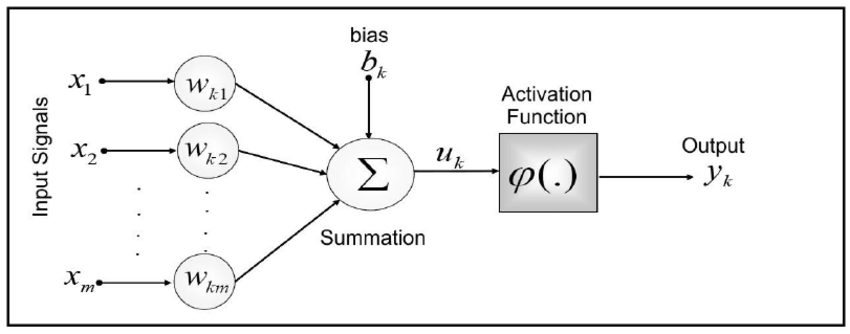
\includegraphics[width= 0.7\linewidth]{bab2/ANN 2.png}
      \caption{\textit{Artificial Neural Network}}
      \label{fig: ANN}
    \end{center}
\end{figure}

Nilai sebuah output dari \textit{artificial neural network} juga
dipengaruhi oleh bias. Bias pada sebuah model dapat disebabkan oleh dataset awal atau karena kurangnya
pemprosesan data. Sebagai contoh, data untuk membedakan gambar kucing dan anjing digunakan untuk membangun
sebuah model klasifikasi anjing dan kucing, terdapat 500 gambar data anjing yang digunakan, namun
hanya ada 20 gambar kucing yang digunakan. Tentunya dengan dataset ini, model akan cenderung
memprediksi atau mengklasifikasikan gambar menjadi kelas anjing. Bias yang sama pun juga dapat terjadi
pada sebuah prediksi nilai atau klasifikasi teks. Bias yang dapat terjadi lainnya adalah jika model
memiliki data \textit{train} duplikat. Hal ini dapat memberikan \textit{overfitting} 
karena saat diuji coba dengan gambar yang berbeda, nilai performa model menurun.

Pada sebuah \textit{artificial neural network} terdapat beberapa \textit{activation function} yang 
dapat diaplikasikan. \textit{Activation function} mengatur apakah sebuah neuron harus diaktifkan dan nilainya
digunakan atau tidak. Hal ini berguna dalam memprediksi ataupun mengkalsifikasi suatu hal berdasarkan
nilai dari input \textit{artificial neural network} dimana dengan sebuah \textit{threshold}, nilai input
tertentu dapat memberikan nilai output 0 jika data input dianggap tidak berguna dalam memprediksi. Terdapat tiga \textit{activation function} yang umum digunakan yaitu fungsi sigmoid, ReLu, dan TanH.

\begin{itemize}
    \item \textbf{Sigmoid}
    \begin{equation}
        h_ \theta (x) =  \frac{\mathrm{1} }{\mathrm{1} + e^- \theta^Tx }
    \end{equation}

    \begin{figure}[h!]
        \begin{center}
          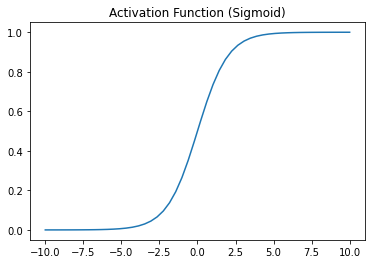
\includegraphics[width= 0.5\linewidth]{bab2/21. sigmoid.png}
          \caption{Fungsi Sigmoid}
          \label{fig: Sigmoid}
        \end{center}
    \end{figure}

    Fungsi aktivasi yang umum digunakan pertama adalah fungsi sigmoid, fungsi sigmoid memberikan
    nilai dibawah 0,5 pada nilai input negatif, dan nilai 0 pada nilai negatif yang lebih kecil dari
    -5. Sebaliknya, fungsi ini memberikan nilai diatas 0,5 pada nilai positif dan nilai 1 pada nilai
    input diatas 5. Jika nilai input 0, maka fungsi ini akan memberikan nilai 0,5. Nilai maksimal dari fungsi
    ini adalah 1 dan nilai minimalnya adalah 0.

    \item \textbf{Tanh}
    \begin{equation}
        \tanh{x}
    \end{equation}

    \begin{figure}[h!]
        \begin{center}
          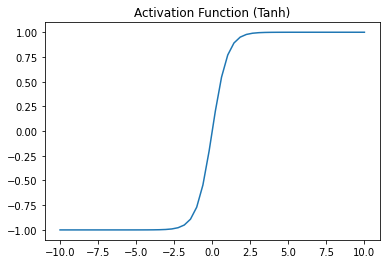
\includegraphics[width= 0.5\linewidth]{bab2/22. tanh.png}
          \caption{Fungsi Tanh}
          \label{fig: Tanh}
        \end{center}
    \end{figure}

    Fungsi aktivasi kedua adalah tanh, jika sebelumnya fungsi sigmoid memiliki nilai minimal 0, maka
    pada fungsi tanh, nilai minimal yang dimiliki adalah -1 sedangkan nilai maksimal yang dimiliki adalah 1. 
    Fungsi tanh akan memberikan nilai negatif pada input negatif, nilai 0 pada input 0, dan nilai 
    positif pada input positif.

    \item \textbf{ReLu}
    \begin{equation}
        Relu(x) = max(0,x)
    \end{equation}

    \begin{figure}[h!]
        \begin{center}
          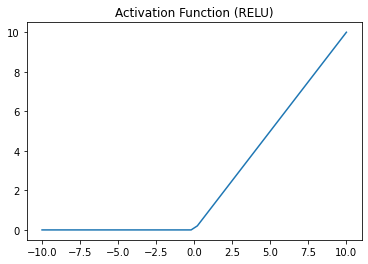
\includegraphics[width= 0.5\linewidth]{bab2/20. Relu.png}
          \caption{Fungsi ReLu}
          \label{fig: ReLu}
        \end{center}
    \end{figure}

    Fungsi aktivasi ketiga adalah ReLu, fungsi ReLu memiliki nilai minimal 0 namun tidak mempunyai nilai maksimal. 
    ReLu merupakan suatu fungsi aktivasi linear yang sering digunakan dalam mengklasifikasi gambar.
    Fungsi ReLu akan memberikan nilai 0 pada input 0 dan negatif sedangkan pada input positif, ReLu akan memberikan
    output nilai input itu sendiri. Terdapat juga fungsi ReLu yang memberikan nilai negatif pada input
    negatif, fungsi ReLu yang memberikan nilai negatif disebut dengan leaky ReLu.

\end{itemize}

\section{\textit{Convolutional Neural Network}}
\textit{Convolutional neural network} adalah sebuah jaringan \textit{neural network} yang memanfaatkan
operasi matematika konvolusi dan pooling dalam memproses matriks atau tensor inputnya.
\textit{Convolutional neural network} umum digunakan dalam pengolahan citra karena dapat mengekstrak
fitur pada gambar dengan baik.

\begin{figure}[h!]
    \begin{center}
      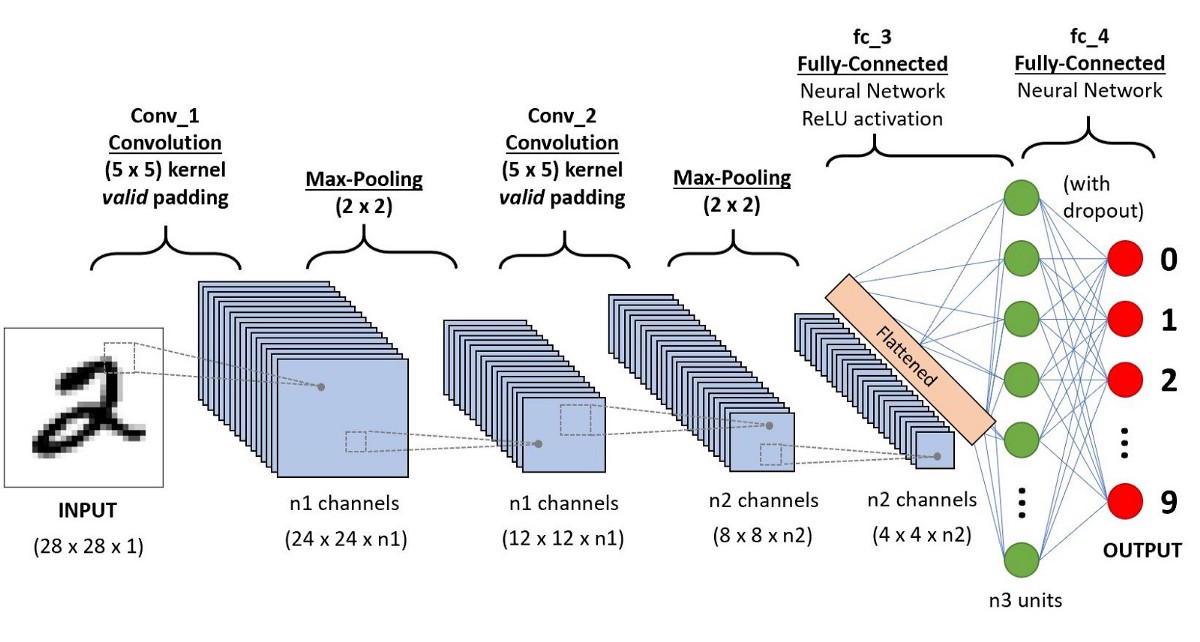
\includegraphics[width= 0.75\linewidth]{bab2/Contoh Arsitektur CNN.jpeg}
      \caption{Contoh Arsitektur CNN}
      \label{fig: Arsi CNN}
    \end{center}
\end{figure}

\subsection{Konvolusi}
Konvolusi merupakan suatu operasi matematika yang sering dilakukan untuk melakukan pemprosesan gambar.
Konvolusi dilakukan untuk mengekstrak fitur-fitur pada gambar agar perbedaan nilai pada fitur yang
ingin diekstrak semakin besar dan fitur yang akan diproses menjadi lebih mudah dilihat oleh komputer
karena memiliki nilai yang lebih besar serta memori atau ukuran gambar yang lebih kecil. Proses konvolusi
dimulai dengan mempersiapkan sebuah matriks kernel yang berukuran sama atau kurang dari ukuran matriks
gambar yang ingin diproses. Umumnya matriks kernel ini berukuran 3x3. Kemudian pada matriks awal akan 
diambil sebuah bagian dari matriks yang berukuran sama kemudian dikalikan dengan matriks kernel. Hasil
dari perkalian tersebut kemudian dijumlahkan menjadi satu nilai yang menjadi satu elemen pada matriks
yang baru / matriks dari hasil konvolusi. Pada CNN, nilai kernel matriks ini akan didefinisikan oleh
\textit{neural network}.

\begin{figure}[h!]
    \begin{center}
      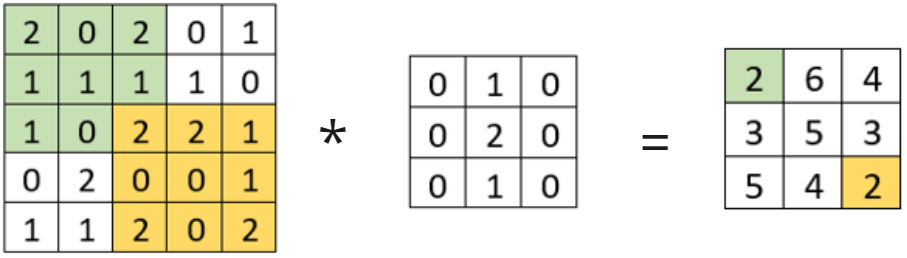
\includegraphics[width= 0.7\linewidth]{bab2/Convolution.png}
      \caption{Konvolusi}
      \label{fig: Konvolusi}
    \end{center}
\end{figure}

\subsection{\textit{Pooling}}
\textit{Pooling} merupakan suatu operasi matematika yang digunakan untuk memperkecil ukuran matriks dengan memilih
atau memproses nilai pada matriks. \textit{Pooling} pada pemprosesan citra umumnya dilakukan pada setiap bagian matriks
dengan ukuran 2x2 atau 3x3. Contoh dari operasi \textit{pooling} dapat dilihat pada gambar \ref{fig: Pooling}.
Terdapat beberapa jenis \textit{pooling}, dan beberapa \textit{pooling} yang sering digunakan ialah
\textit{max pooling} dan \textit{average pooling}. \textit{Max pooling} mengambil elemen matriks dengan
nilai tertinggi pada suatu sekumpulan matriks sesuai dengan ukuran yang sudah didefinisikan. Misalnya 
jika matriks berukuran 4x4 mengalami proses \textit{pooling} 2x2, maka hasil dari matriks tersebut adalah
1 elemen matriks dari setiap bagian matriks berukuran 2x2 pada matriks 4x4 dimana elemen yang telah diproses
tidak diproses kembali. Sehingga hasil dari matriks 4x4 yang mengalami proses \textit{pooling} 2x2
adalah matriks berukuran 2x2.

Sedangkan jenis \textit{pooling} yang sering digunakan lainnya adalah \textit{average pooling}
dimana jika sebelumnya pada \textit{max pooling} elemen dengan nilai tertinggi yang dipilih, maka
pada \textit{average pooling} maka akan dipilih nilai rata-rata dari \textit{pooling} tersebut. Jika
misalnya pada sebuah matriks dilakukan proses \textit{pooling} 2x2, maka rata-rata dari empat elemen
dari bagian matriks yang berukuran 2x2 akan menjadi elemen dari matriks hasil \textit{pooling}. Perbedaan 
jenis \textit{pooling} tidak mempengaruhi ukuran matriks dari hasil pemprosesan \textit{pooling}, namun
tentunya mempengaruhi nilai hasil \textit{pooling}.

\begin{figure}[h!]
    \begin{center}
      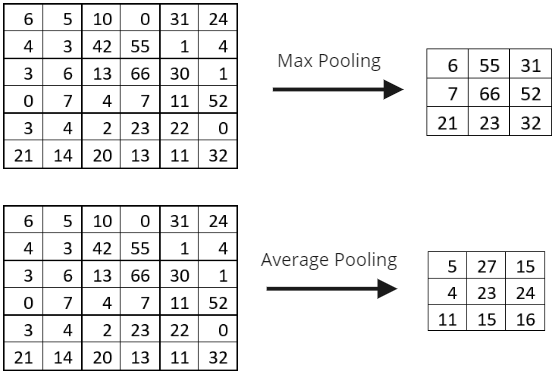
\includegraphics[width= 0.7\linewidth]{bab2/Pooling.png}
      \caption{Contoh \textit{Pooling} 2x2}
      \label{fig: Pooling}
    \end{center}
\end{figure}

\section{Deteksi Objek}
Deteksi objek (\textit{object detection}) adalah suatu teknik pada \textit{computer vision} dimana
suatu komputer dapat mengenali dan mengetahui lokasi dari objek yang menjadi fokus secara otomatis
layaknya manusia. \textit{Object detection} dapat dicapai dengan penggunaan \textit{deep learning}.
Salah satu kelemahan dalam pembuatan sebuah komputer pendeteksi objek adalah, tingginya daya komputasi
yang diperlukan dan dalam mendeteksi \textit{multiple class} membutuhkan dataset yang banyak sehingga
kebutuhan \textit{storage} pun meningkat. Sebagian besar detektor objek beroperasi dengan memilih 
sekumpulan kandidat region yang mengandung objek fokus dari gambar dan mengklasifikasikannya ke dalam 
daerah objek \textit{foreground} dan daerah yang tidak memiliki objek (biasanya disebut sebagai latar belakang). 
Pada dasarnya, pendekatan tersebut dapat mengurangi tugas deteksi objek menjadi tugas klasifikasi gambar yang lebih sederhana. 
Kandidat daerah yang akan diklasifikasikan dapat diperoleh dengan mudah dengan cara 
\textit{brute force} dengan menggeser jendela m × n di atas gambar atau yang sering disebut algoritma 
\textit{sliding window}. Mengikuti metode ekstraksi fitur dari \textit{sliding window}, terdapat metode dimana setiap 
\textit{region} akan dinilai berdasarkan kerapatan tepi, ukuran, dan lokasi pada objek dan metode lain
dimana gambar tersebut akan disegmentasi terlebih dahulu menjadi beberapa bagian kemudian mengkombinasikannya
berdasarkan kemiripannya. Salah satu metode yang mensegmentasi gambar dan mengelompokkan gambar tersebut adalah
\textit{selective search} \cite{UijlingsIJCV2013}. 

Dalam menunjukkan lokasi objek, seringkali sebuah \textit{bounding box} dibentuk untuk menandakan lokasi
dari objek yang menjadi fokusan. \textit{Bounding box} juga digunakan dalam metode \textit{selective search}
untuk menjadi kandidat objek deteksi. Kandidat objek harus meliputi semua objek pada gambar sehingga
tidak ada objek yang terlewati dan objek-objek tersebut dapat diklasifikasi. Di sisi lain
\textit{bounding box} pada kandidat objek yang terlalu banyak dapat mengakibatkan \textit{bounding box}
menimpa satu sama lain pada satu objek yang sama. 

Untuk mengatasi hal ini dan mengambil \textit{bounding box}
terbaik, maka suatu metode yang dinamakan \textit{non-max supression} per diaplikasikan. Pertama-tama, 
semua \textit{bounding box} perlu dicek apakah menimpa objek yang sama atau tidak, hal ini dapat dilakukan
dengan menganalisa koordinat dari \textit{bounding box}, kemudian nilai \textit{interference over union} (IoU)
pada \textit{bounding box} yang meliputi objek yang sama akan diperiksa, jika nilai IoU pada
\textit{bounding box} di atas 0,5 maka \textit{bounding box} tersebut tidak dibuang kemudian jika terdapat
beberapa \textit{bounding box} yang memiliki nilia IoU di atas 0,5, maka akan dipilih \textit{bounding box}
dengan nilai IoU terbesar \cite{hawking1988}.

\begin{figure}[h!]
    \begin{center}
      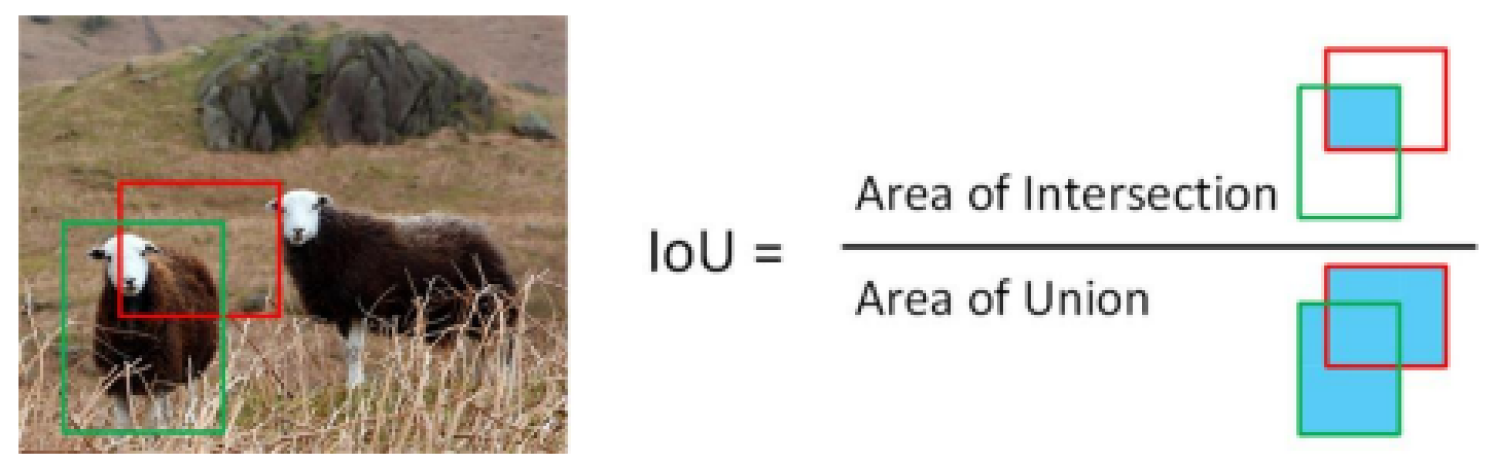
\includegraphics[width= 1\linewidth]{bab2/IoU.png}
      \caption{\textit{Intersect over Union}}
      \label{fig: IoU}
    \end{center}
\end{figure}

\subsection{\textit{Two-Stage Object Detectors}}
\textit{Two-stage object detectors} adalah suatu prinsip pada deteksi objek dengan mengikuti prinsip
mencari daerah kandidat atau daerah proposal. Kemudian daerah proposal tersebut akan dideteksi secara
lebih lanjut. Seperti namanya \textit{two stage object detectors} memiliki dua tahapan detektor
dimana tahap pertama adalah pemberian proposal dan tahap kedua adalah klasifikasi dan deteksi objek
\cite{hawking1988}.

Salah satu contoh algoritma yang menerapkan \textit{two-stage object detectors} adalah R-CNN. 
Pada R-CNN, algoritma pencarian selektif mengekstrak \textit{{region proposal}}
dari gambar, yang kemudian akan menghasilkan satu set kandidat objek yang diberi \textit{bounding box}. 
Setelah memperoleh proposal wilayah, jaringan saraf convolutional digunakan sebagai ekstraktor fitur 
di atas setiap proposal yang diekstraksi, menghasilkan \textit{feature} gambar dari setiap proposal. 

\begin{figure}[h!]
    \begin{center}
      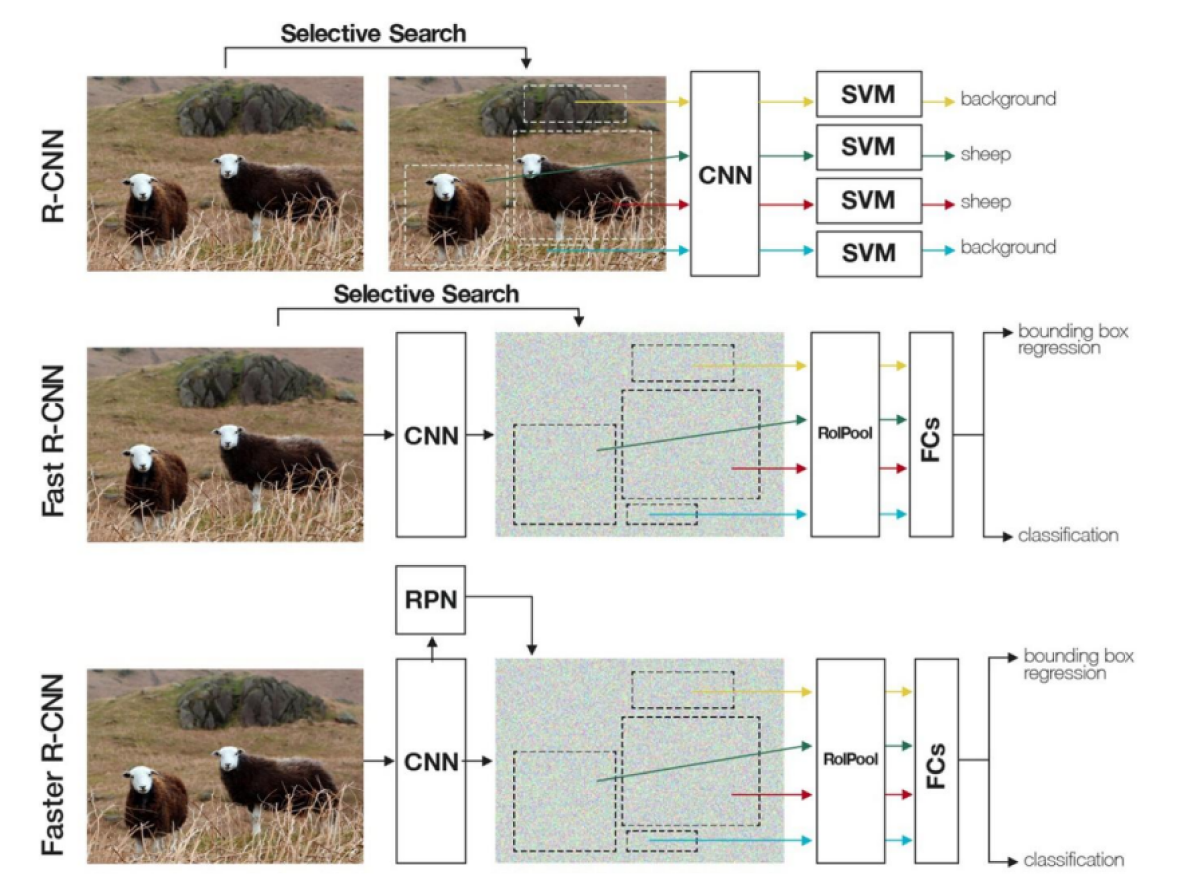
\includegraphics[width= 1\linewidth]{bab2/Two stage.png}
      \caption{Contoh \textit{Two Stage Detector}}
      \label{fig: Two Stage Detector}
    \end{center}
\end{figure}

Secara khusus, untuk setiap gambar, pembuatan \textit{region proposal} yang membentuk sebuah
\textit{bounding box} suatu objek harus mempunyai IoU melebihi nilai ambang (0,5 umumnya digunakan). Hal ini 
dianggap sebagai contoh positif untuk kelas objek yang sesuai,
sementara proposal yang memiliki nilai IoU
lebih rendah dari ambang (0,5) dianggap sebagai contoh negatif untuk semua kelas objek dan dianggap 
sebagai latar belakang (bukan objek). Setelah proposal dibentuk, maka algoritma lanjutan yang menggunakan SVM akan memprediksi kelas pada
objek yang menjadi proposal dan objek proposal yang dipilih adalah proposal yang memiliki IoU tertinggi
dari suatu objek yang tumpang tindih.

\subsection{\textit{Single-Stage Object Detector}}
Selain \textit{two-stage object detector} adapula deteksi objek dengan menggunakan \textit{single stage}.
Pada metode ini, \textit{region proposal} tidak dibentuk sehingga objek dideteksi dan diklasifikasi
secara langsung. Tentunya karena tidak memerlukan tahapan pemebentukan \textit{region proposal} maka
algoritma yang menggunakan metode ini memproses gambar lebih cepat dan mendeteksi objek secara lebih cepat.
Beberapa contoh dari penerapan \textit{Single-stage object detector} adalah algoritma 
\textit{Single Shot Detector (SSD)} dan \textit{You Only Look Once (YOLO)} 
\cite{https://doi.org/10.48550/arxiv.1506.02640}. 

YOLO menggunakan 24 lapis jaringan konvolusi untuk ekstraksi fitur, diikuti oleh 2 lapisan yang 
\textit{fully connected}. 20 lapisan konvolusional pertama dilatih pada ImageNet untuk klasifikasi, 
dan setelah menambahkan lapisan yang tersisa, model selanjutnya dilatih untuk mendeteksi objek. 
YOLO membagi gambar menjadi sel menjadi ukuran SxS (umumnya 7x7) dan memprediksi kotak pembatas 
bersama dengan skor \textit{confidence}, serta distribusi probabilitas kelas untuk setiap sel grid. 
Setiap pembatas kotak diberikan parameter oleh titik pusat kotak relatif terhadap sel grid, yang
lebar dan tingginya relatif terhadap keseluruhan gambar \cite{hawking1988}. Skor kepercayaan dari kotak pembatas secara 
formal didefinisikan sebagai IoU antara kotak pembatas yang diprediksi dan
kotak kebenaran dasar yang sesuai. Perhatikan bahwa tidak seperti Faster R-CNN yang memprediksi 
offset dari kotak jangkar, YOLO memprediksi koordinat kotak pembatas akhir secara langsung.

\begin{figure}[h!]
    \begin{center}
      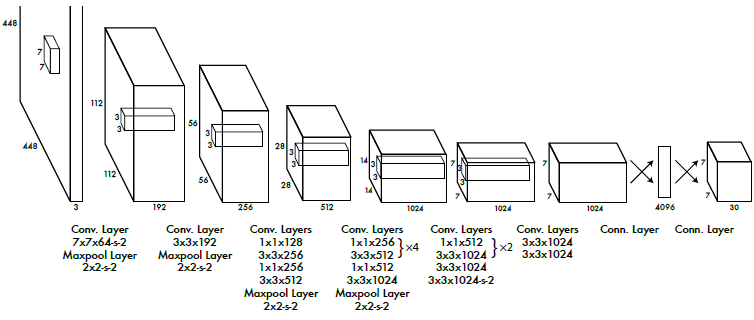
\includegraphics[width= 1\linewidth]{bab2/Yolo Archi.png}
      \caption{Arsitektur YOLO \cite{YOLOYOLA}}
      \label{fig: Archi YOLO}
    \end{center}
\end{figure}

\section{Algoritma Deteksi Objek Mask R-CNN}

Mask R-CNN \cite{https://doi.org/10.48550/arxiv.1703.06870} adalah jaringan saraf dalam untuk memecahkan masalah segmentasi instans. 
Dengan kata lain, dapat memisahkan objek yang berbeda dalam gambar atau video. 
Dengan memberikan input gambar, Mask R-CNN akan memberikan kotak pembatas objek, kelas, dan \textit{mask}.
Mask R-CNN merupakan pengembangan dari \textit{faster R-CNN} dimana sebuah \textit{mask} akan dibentuk
dalam mendeteksi objeknya.

Saat ini Mask R-CNN pertama kali dikemukakan pada tahun 2017 dan sejak saat itu menjadi salah satu algoritma
deteksi objek yang terkenal dan menarik untuk diimplementasikan. Pengaplikasian Mask R-CNN sudah dilakukan
di berbagai penelitian seperti deteksi algae, deteksi sel kanker, deteksi pneumonia, dan masih banyak lagi.
Mask R-CNN adalah salah satu algoritma yang memanfaatkan \textit{two stage detector} dalam mendeteksi objek
dan dapat mensegmentasi objek hingga level piksel.

\begin{figure}[h!]
    \begin{center}
      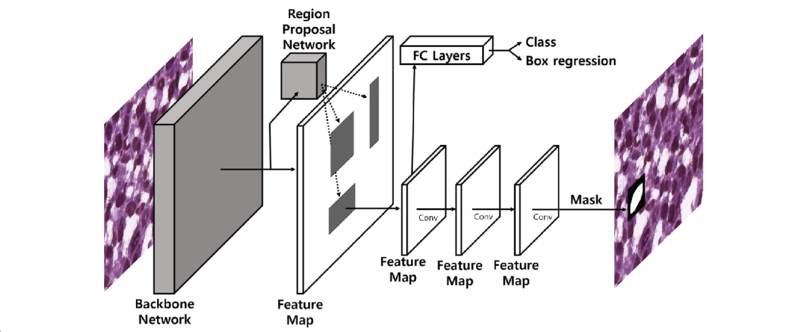
\includegraphics[width= 1\linewidth]{bab2/Mask R-CNN Archi.png}
      \caption{Arsitektur Mask R-CNN \cite{Mask-archi}}
      \label{fig: Mask RCNN Archi}
    \end{center}
\end{figure}

Ada dua tahap Mask RCNN. Pertama, menghasilkan proposal tentang wilayah di mana mungkin terdapat objek 
berdasarkan gambar input. Kedua, memprediksi kelas objek, menyempurnakan kotak pembatas dan 
menghasilkan \textit{mask} di tingkat piksel objek berdasarkan proposal tahap pertama.
Tentunya seperti algoritma deteksi objek lainnya, pelabelan kelas dan penunjukkan lokasi objek
yang ingin dideteksi dibutuhkan pada data \textit{train}. Mask R-CNN mengambil data kelas dan objek
yang telah diberikan \textit{mask} kemudian mengekstrak fitur-fitur pada gambar data \textit{train}.

Dalam mengambil target untuk melatih proses pengekstrakan fitur secara lebih dalam, maka sebuah target
perlu dibentuk. Pada hal ini, Mask R-CNN memanfaatkan \textit{anchor box} untuk memberikan perkiraan
dimanakah objek yang perlu dideteksi berada, jika \textit{anchor box} mempunyai IoU lebih dari sama dengan 0,5
dengan \textit{bounding box} awal maka \textit{anchor box} tersebut disimpan untuk menjadi target
kecuali jika \textit{bounding box} tersebut \textit{overlap} dengan \textit{anchor box} lain, maka
\textit{anchor box} yang mempunyai nilai IoU terbaik yang akan dipilih menjadi target.
\textit{Anchor box} yang disimpan akan menjadi target bagi \textit{backbone} untuk mengekstrak fitur
menggunakan neural network.

Pengekstrakan fitur dimulai dengan proses konvolusi pada jaringan \textit{backbone}. Umumnya
\textit{backbone} yang digunakan pada algoritma ini adalah \textit{Residual Network} atau yang 
disingkat ResNet. ResNet merupakan sebuah jaringan yang dibentuk oleh berbagai konvolusi, proses
\textit{pooling}, dan lapisan neural network. Saat ini terdapat lima layer atau lima jenis ResNet
yang dibedakan menurut jumlah layernya. Untuk 18 layer ResNet, jaringan tersebut disusun oleh 1 layer
konvolusi 7x7-64 neural network, kemudian proses pooling 3x3 (tidak dihitung sebagai layer), kemudian
4 layer konvolusi 3x3-64 neural network, 4 layer konvolusi 3x3-128 neural network, 4 layer konvolusi 3x3-256 neural network,
4 layer konvolusi 3x3-512 neural network, dan layer terakhir adalah \textit{fully connected layer}
atau yang disebut sebagai FC dengan \textit{softmax function} untuk memberikan output dengan berbagai kelas.

Sedangkan pada contoh layer ResNet yang lain, contohnya ResNet 101, layer pada ResNet akan terdiri
dari 101 layer dan dapat dilihat pada gambar \ref{fig: Resnet macam}. Jaringan pada \textit{backbone}
akan menghasilkan sebuah \textit{Region Proposal Network (RPN)} yang merupakan hasil dari \textit{anchor box}
yang mempunyai IoU lebih besar dari 0,5 dengan \textit{bounding box} asli. Dan \textit{feature map} 
yang memuat data hasil dari konvolusi dan pelatihan \textit{neural network} yang berada pada \textit{backbone}.

\begin{figure}[h!]
    \begin{center}
      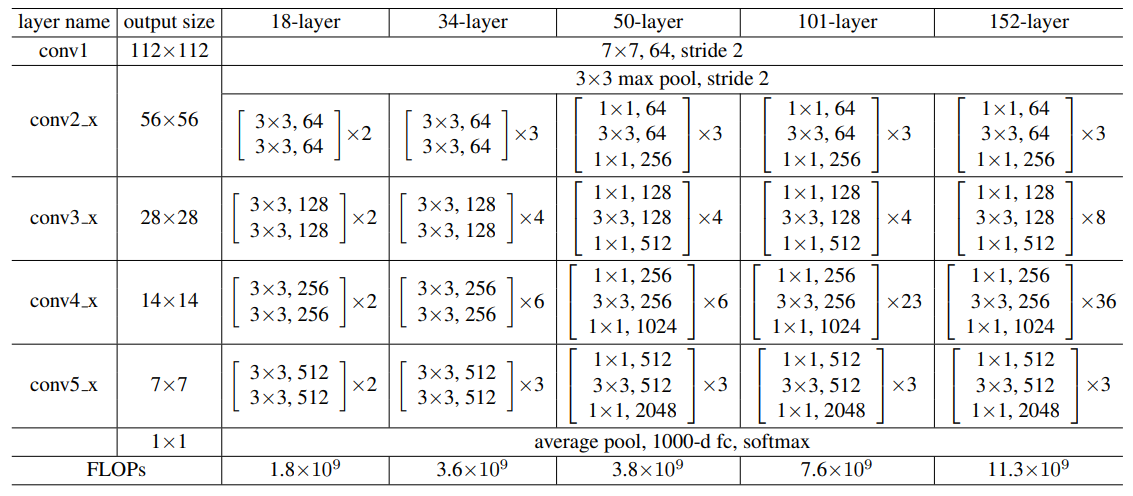
\includegraphics[width= 1\linewidth]{bab2/ResNet 101-2.png}
      \caption{Macam - macam \textit{Residual Network (ResNet)} \cite{https://doi.org/10.48550/arxiv.1512.03385}}
      \label{fig: Resnet macam}
    \end{center}
\end{figure}

Hasil dari ekstraksi fitur oleh jaringan \textit{backbone} berupa sebuah \textit{heatmap} hasil konvolusi
dari algoritma ResNet yang disebut \textit{feature map}, hal ini akan memudahkan tahapan memprediksi kelas, ukuran objek, dan pembuatan \textit{mask}.
Dalam memprediksi kelas dan memberikan \textit{bounding box} pada objek, \textit{feature map} diproses
menggunakan \textit{fully connected layer}. \textit{Fully connected layer} merupakan sebuah lapisan
\textit{neural network} yang mengkoneksikan setiap neuron pada satu layer ke setiap neuron pada layer selanjutnya
umumnya digunakan pada lapisan output untuk memberikan kelas. Selain itu, \textit{feature map} juga digunakan
untuk membentuk \textit{mask} menggunakan lapisan konvolusi.

Dalam melatih model Mask R-CNN, terdapat beberapa metriks yang perlu diketahui untuk mengetahui
seberapa bagus proses \textit{training} yang biasanya dinyatakan dalam metriks loss. dalam Mask RCNN
terdapat 5 metriks loss yang dibedakan menjadi loss RPN dan loss MRCNN. Loss RPN merupakan loss yang terjadi pada pembuatan dan pelatihan jaringan \textit{backbone}
dalam memberikan \textit{region proposal}. Loss RPN dibedakan menjadi dua yaitu loss RPN \textit{bounding box}
dan loss RPN \textit{class}. Loss RPN \textit{bounding box} merupakan loss yang terjadi untuk mengetahui
seberapa besar perbedaan \textit{bounding box} pada objek yang diprediksi dengan \textit{bounding box}
aslinya. Sedangkan pada Loss RPN class merupakan loss yang terjadi saat ada kesalahan prediksi objek menjadi
\textit{background} ataupun prediksi \textit{background} menjadi objek.

\begin{equation}
    \label{eq :loss}
    \mathcal{L} = \mathcal{L}_\text{RPN-cls} + \mathcal{L}_\text{RPN-box}
\end{equation}

\begin{equation}
    \label{eq :cls_loss}
    \mathcal{L}_\text{RPN-cls} (p_i, p^*_i) = - p^*_i \log p_i - (1 - p^*_i) \log (1 - p_i)
\end{equation}

\begin{equation}
    \label{eq :bbox loss}
    \mathcal{L}_\text{RPN-box} = \frac{\lambda}{N_\text{box}} \sum_i p^*_i \cdot L_1^\text{smooth}(t_i - t^*_i)
\end{equation}

Kemudian dalam loss yang sering kali disebut loss MRCNN merupakan loss yang terjadi tahapan setelah
pembuatan \textit{feature map} dan digunakan untuk mengetahui seberapa bagus performa dari output
pada Mask RCNN. Loss MRCNN dibedakan menjadi tiga jenis yaitu loss class, loss bounding box, dan loss mask.
\textit{loss class} adalah loss yang terjadi saat adanya kesalahan prediksi pada kelas objek, jika sebelumnya
pada loss rpn, perbedaan kelas hanyalah objek atau tidak (\textit{foreground or background}) pada loss
MRCNN, kelas yang diprediksi adalah kelas nama objek yang diteliti. Kemudian pada loss bounding box
merupakan hal yang hampir sama pada loss rpn bounding box, perbedaannya ialah, loss ini merupakan
perbandingan output akhir prediksi dengan data awal. Kemudian loss terakhir adalah loss mask yang merupakan
metriks untuk melihat seberapa berbedanya mask yang dibentuk dengan mask data awal. Dibawah ini merupakan
persamaan dari loss MRCNN.

\begin{equation}
    \label{eq :loss}
    \mathcal{L} = \mathcal{L}_\text{cls} + \mathcal{L}_\text{box} + \mathcal{L}_\text{mask}
  \end{equation}
  
  \begin{equation}
    \label{eq:other Loss}
    \mathcal{L}_\text{fr} = \mathcal{L}_\text{cls} + \mathcal{L}_\text{box}
  \end{equation}
  
  \begin{equation}
    \mathcal{L}_\text{fr}(\{p_i\}, \{t_i\}) = \frac{1}{N_\text{cls}} \sum_i \mathcal{L}_\text{cls} (p_i, p^*_i) + \frac{\lambda}{N_\text{box}} \sum_i p^*_i \cdot L_1^\text{smooth}(t_i - t^*_i)
  \end{equation}
  
  \begin{equation}
    \label{eq :cls_loss}
    \mathcal{L}_\text{cls} (p_i, p^*_i) = - p^*_i \log p_i - (1 - p^*_i) \log (1 - p_i)
  \end{equation}
  
  \begin{equation}
    \label{eq :bbox loss}
    \mathcal{L}_\text{box} = \frac{\lambda}{N_\text{box}} \sum_i p^*_i \cdot L_1^\text{smooth}(t_i - t^*_i)
  \end{equation}
  
  \begin{equation}
    \label{eq :mask loss}
    \mathcal{L}_\text{mask} = - \frac{1}{m^2} \sum_{1 \leq i, j \leq m} \big[ y_{ij} \log \hat{y}^k_{ij} + (1-y_{ij}) \log (1- \hat{y}^k_{ij}) \big]
\end{equation}

\section{Metode Analisa Performa Model}
Terdapat beberapa metode yang bisa dilakukan untuk mengetahui apakah suatu model memiliki akurasi yang cukup. 
Penelitian ini menggunakan beberapa formula yang sudah ditentukan seperti \textit{recall, precision, f1-score} 
dan \textit{confusion matrix}.

\subsection{\textit{Recall}}
\textit{Recall} adalah formula yang harus digunakan ketika kita memiliki data yang tidak seimbang. Berbeda 
dengan akurasi yang hanya menghitung persentase model memprediksi hasil yang sesuai dengan label secara 
keseluruhan, \textit{recall} akan menghitung rasio nilai yang diprediksi positif dengan total keseluruhan 
nilai yang positif \cite{metrics_ml}. Rumus \ref{form:recall} merupakan rumus untuk menghitung \textit{recall}.

\begin{equation}
    Recall = \frac{TP}{TP+FN}
    \label{form:recall}
\end{equation}

\subsection{\textit{Precision}}
Seringnya, kita tidak hanya melihat tingkat akurasi suatu model hanya dengan besaran \textit{recall} maupun 
tingkat akurasi nya. \textit{Precision} adalah formula untuk menghitung rasio dari prediksi TP (\textit{True 
Positive}) yang benar dengan keseluruhan prediksi. Apabila prediksi yang dilakukan oleh model kita ternyata 
memiliki tingkat presisi yang tinggi namun memiliki tingkat \textit{recall} yang rendah, ada kemungkinan model 
tidak dapat melakukan prediksi pada data yang bersifat negatif \cite{metrics_ml}. Rumus \ref{form:precision} 
merupakan rumus untuk menghitung nilai dari \textit{precision} suatu model.

\begin{equation}
    Precision = \frac{TP}{TP+FP}
    \label{form:precision}
\end{equation}

Baik \textit{recall} maupun \textit{precision} merupakan nilai yang cukup penting terutama pada data yang tidak 
seimbang. Terdapat 3 kelfndisi yang umum terjadi pada saat membandingkan antara \textit{precision} dengan 
\textit{recall}.

\begin{itemize}
    \item \textit{Recall} tinggi, \textit{Precision} rendah
          Sebagian besar data positif dapat diprediksi dengan benar (\textit{False Negative} yang Rendah), 
          namun hanya ada sebagian kecil data negatif yang diprediksi dengan benar (\textit{True Negative} 
          rendah).

    \item \textit{Recall} rendah, \textit{Precision} tinggi
          Hasil prediksi model memiliki banyak sekali prediksi negatif (\textit{False Negative} tinggi), 
          namun apabila digunakan untuk memprediksi data positif, maka hasil prediksi sebagian besarnya adalah 
          benar (\textit{False Positive} rendah).

    \item \textit{Recall} tinggi, \textit{Precision} tinggi
          Merupakan hasil yang ideal dalam pembuatan model pembelajaran mesin. Disini didapatkan bahwa baik 
          hasil prediksi untuk data positif maupun hasil prediksi untuk data negatif sebagian besarnya adalah 
          benar (\textit{True Positive} dan \textit{True Negative} tinggi).

\end{itemize}

\subsection{mAP@50}
Dalam mengukur performa sebuah deteksi objek, sebuah threshold IoU 0,5 merupakan parameter yang umum digunakan
dimana jika IoU deteksi bernilai lebih dari sama dengan 0,5, maka dapat dikatakan bahwa deteksi yang
dihasilkan adalah bagus. Adapula parameter performa yang dinamakan \textit{average precission} yang didefinisikan
sebagai luasan dari area di bawah kurva \textit{recall-precission}. Umumnya parameter performa ini ditulis
sebagai mAP@50

\subsection{\textit{F1-Score}}

\textit{F1-Score} adalah besaran yang berasal dari rata - rata harmonik dari \textit{recall} dan 
\textit{precision}. Rata  - rata harmonik dipilih karena akan menghasilkan nilai rata - rata yang lebih rendah 
dalam kondisi tidak seimbang apabila dibandingkan dengan rata - rata aritmatis biasa. Dengan rata - rata seperti 
itu, suatu model dapat menjadi lebih rentan terhadap bias dan memudahkan pada saat pembuatan model 
\cite{metrics_ml}. Rumus \ref{form: f1-score} merupakan rumus untuk menghitung f1-score.

\begin{equation}
    \label{form: f1-score}
    F1-Score = 2 \times \frac{\textit{Recall} \times \textit{Precision}}{\textit{Recall} + \textit{Precision}}
\end{equation}

\subsection{\textit{Confusion Matrix}}

\textit{Confusion Matrix} adalah tabel kesimpulan yang berisi jumlah prediksi baik yang benar maupun yang 
salah dan nilai label baik yang benar maupun salah. Biasanya tabel jenis ini digunakan untuk tugas yang 
bersifat klasifikasi dan berfungsi untuk memvisualisasi bagaimana suatu performa model dalam suatu dataset.

\begin{table}
    \caption{Contoh \textit{Confusion Matrix}}
    \label{tab:cth_confusion_mtrx}
    \centering
    \begin{tabular}{|l|l|l|l|l}
        \cline{1-4}
        \multicolumn{2}{|l|}{\multirow{2}{*}{}} & \multicolumn{2}{l|}{\textbf{Aktual}} &                \\ \cline{3-4}
        \multicolumn{2}{|l|}{}                  & Positif                              & Negatif &      \\ \cline{1-4}
        \multirow{2}{*}{\textbf{Prediksi}}      & Positif                              & TP      & FP & \\ \cline{2-4}
                                                & Negatif                              & FN      & TN & \\ \cline{1-4}
    \end{tabular}
\end{table}

Tabel \ref{tab:cth_confusion_mtrx} adalah contoh tabel \textit{confussion matrix} untuk prediksi dengan 2 label. 
Apabila melihat pada tabel tersebut, dapat terlihat bahwa jumlah prediksi dipecah menjadi masing - masing kelas. 
Diharapkan dengan dipecah menjadi beberapa kelas seperti itu, akan membuat proses pengujian lebih mudah karena 
akan lebih mudah melihat pada saat model memprediksi jenis data apa yang masih memiliki tingkat akurasi yang 
kurang bagus. Terdapat beberapa hal yang harus diketahui untuk dapat memahami sebuah tabel \textit{confussion 
matrix}, yaitu :

\begin{itemize}[nolistsep]
    \item Positif (P)
          Berisi data yang bernilai positif, baik data tersebut beasal dari hasil prediksi maupun data aktual 
          yang didapat dari dataset.

    \item Negatif (N)
          Berisi data yang bernilai negatif, baik data tersebut berasal dari hasil prediksi maupun data aktual 
          yang didapat dari dataset.

    \item \textit{True Positive} (TP)
          Suatu kondisi dimana baik hasil prediksi maupun data aktual sama - sama bernilai positif. Semakin 
          tinggi nilai dari TP, semakin akurat pulalah model yang sudah dibuat.

    \item \textit{False Positive} (FP)
          Suatu kondisi dimana hasil prediksi adalah positif, namun pada data aktual bernilai negatif. 
          Biasanya, semakin tinggi nilai dari FP ini, maka model semakin memilki kecenderungan untuk 
          mengeluarkan nilai positif dibanding negatif atau terjadinya bias pada model.

    \item \textit{True Negative} (TN)
          Suatu kondisi dimana hasil prediksi dan data aktual bernilai negatif. Semakin tinggi nilai FN 
          berarti semakin akurat model yang sudah dibuat.

    \item \textit{False Negative} (FN)
          Suatu kondisi dimana hasil prediksi adalah negatif, namun pada data aktual bernilai positif. 
          Biasanya, semakin tinggi nilai dari TN ini, maka model semakin memiliki kecenderungan untuk 
          mengeluarkan nilai negatif dibanding positif.

\end{itemize}

%%%%%%%%%%%%%%%%%%%%%%%%%%%%%%%%%%%%%%%%%%%%%%%%%%%%%%%%%%



